The generated mesh from PC2B may still need additional cleanup and detail. The mesh topology is dependant on the meshing algorithm used, naturally. It might not be ideal for an artist to have thousands of polygons build up a surface that could be represented by only one polygon. Furthermore, the laser scanner beam cannot sample reflective or transparent structures, such as windows. Therefore it can only provide artists a reference for manual tracing.

\section{Modeling the current Pellerhaus facade}

The lower part of the current Pellerhaus facade is very similar, almost identical, to the historic one. Thus modeling the modern facade based on LiDAR, photogrammetry, and photographic reference appeared to make sense.

\subsection{Using the PC2B converter software}

First, the LiDAR data was preprocesed in PC2B. We created five scans on location, so all the scans have been meshed with PC2B and imported into Blender. A manual registration of the scans was necessary in Blender, because the scans have been aquired at different locations. Fortunately, all the scans were oriented similarly due to the compass sensor in the laser scanner, and the Pellerhaus facade was a good reference point to align them with each other.

It turned out that the workflow for artists is relatively straightforward. Each scan took approximately 5 minutes to be processed by PC2B. Importing the results in Blender worked flawlessly and created all the necessary data blocks, like the named object and texture. We noticed that distinct names for the panorama textures need to be used to avoid multiple uses of one texture in different scans. The mesh is very helpful to get a sense of the scale of objects and, where the detail is not sufficient, the texture information can help in finding details. Moreover, due to the clear texture, the artist can select unnecessary polygons by simply choosing them from the image texture coordinates (which are usually called UV's in 3D applications) and delete them (see Section \ref{section_texture_coordinates_and_normals}). Other meshing algorithms, such as the Delaunay Tetrahedralization, create textures with very small UV islands and store them efficiently (see Appendix \ref{appendix_delaunay_texture_maps}).

All in all, PC2B generated a mesh that was helpful for tracing. This is how the imported scans looked in Blender:

\begin{figure}[h]
	\centering
	\includegraphics[width=1.0\textwidth]{Production_CombinedLaserScans.png}
	\caption{The manually registered LiDAR scans of the Pellerhaus}
	\label{fig:production_laser_scans_combined}
\end{figure}




\subsection{Using UAV references with photogrammetry}

Unmanned Aerial Vehicles (UAV's, or simply drones) are becoming affordable, and this is true even for very good quality models. In our research we use the DJI Phantom 2 with a GoPro Hero 4 Black mounted on a 3-axis DJI Zenmuse H3-3D Gimbal to create photographic aerial references of the Pellerhaus Nürnberg.\\

Flying a drone legally is not as easy, as one might initially assume. Before even being able to take off with a UAV, German law requires general permission just to enter the air space. In addition, every UAV pilot needs UAV insurance.\\

Regarding the usage of drones inside the city center of Nuremberg, there are more restrictions. The city center of Nuremberg is covered by a controlled air space. Flying in that air space is not permitted until the initial permission from the bavarian aviation authority and UAV insurance are upgraded to commercial versions. Furthermore, pilots need a clearance from Air Traffic Control (ATC). Additionally, the starting and landing procedure requires cordoning off of pedestrians and a special license from the traffic authority. Lastly, the owner of the property needs to be asked for permission to allow the takeoff and landing of the aircraft.\\

\pagebreak

Luckily there are some laws that permit video shoots and photography. For example, the Freedom of Panorama Law (§ 59, German Urheberrechtsgesetz) allows taking photos from pavements and roads permanently located in a public place. This right to freely take and share photographs of buildings and works of public art was almost abolished on July 9th, 2015 by the European Parliament (see Blacker 2015 \parencite{freedomOfPanoramaUnderAttack}). Fortunately, members of the European Parliament have voted against this controversial EU plan (see Cheesman 2015 \parencite{freedomOfPanoramaSaved}) with an overwhelming majority. We would expect immense consequences for historic documentation of buildings if this would have happened.\\

In total we made three flights on location. We planned to use the second flight for single photos shot in an interval of 1 second whereas the other two flights were videos in 4K. Unfortunately, it turned out that the third flight wasn't recorded at all and the second flight was captured as a video file. Luckily we noticed the third video missing while still on location, with a bit of battery life left and about one hour left to use the air space, so we made at least two impressive aerial shots before ending the mission.\\

Having video files instead of still images, the files needed to be exported as still frames to be able to be processed by the software. We tried both the free "Visual SfM" and commercial "Agisoft Photoscan Pro" software solutions to generate additional colored meshes of the Pellerhaus. The total processing time was about 20 hours for Visual SfM and 40 hours for Photoscan to get a 3D point cloud from the images. Comparing the results we noticed that Visual SfM generated a bend facade while Photoscan Pro kept it very straight. Although not recommended (see Balletti et al. 2014 \parencite{calibration_of_action_cameras}), we used a GoPro camera with a short focal length and thus a strong lens distortion for 3D reconstruction. We can confirm that the use of this camera type is not a good choice, since the radial distortion can produce errors in the feature matching phase of photogrammetry. Still, the output should be a good reference for the rough shape of the reconstructed object. If available, LiDAR data should be preferred over Photogrammetry for accurate building reconstruction.

\subsection{Using reference images}

In addition to the LiDAR data and Photogrammetry models, photos were taken on location for additional reference. Very small details can be inspected in photographs while creating an accurate surface. Based on the versatile data available, the model was built up slowly, first by creating the rough shapes for the building and then constantly refining them to get the final model.

\pagebreak

\section{Modeling the historic Pellerhaus facade}

Based on the modern facade it was possible to get a good feel for the size of the Pellerhaus in the Renaissance. Still the main parts above the ground floor of the facade differ dramatically from the modern one. They can only be extracted from photographs.


\subsection{Using historic images as guide}

\begin{wrapfigure}{r}{0.5\textwidth}
	
	\centering
	
	\includegraphics[scale=0.1]{Production_Pellerhaus_1601_Entwurf_6.jpg}
	\hbox{\scriptsize Credit: Altstadtfreunde Nürnberg e.V.}
	\caption{Early draft of the Pellerhaus facade of around 1601}
	\label{fig:production_pellerhaus_draft}
	\vspace{-10pt}
	
\end{wrapfigure}

It is quite lucky that the Pellerhaus history has been documented by an enormous amount of pictures. A fascinating number of about 190 pictures has been provided for free through the association Altstadtfreunde Nürnberg e.V., not including about 100 additional pictures depicting the space in front of the building, to be used in this research.\\

This collection contains a few early drafts of the facade, likely created in the year 1601. Frontal, side or top views are best suited for modeling, especially when they are orthogonal (not distorted by perspective).\\

The modeling process began with adjusting the size of the image to the current Pellerhaus provided by LiDAR. The ground floor of the modern Pellerhaus was duplicated and served as the first guide for the creation of the upper floors. Floor by floor, bottom to top, was modelled by tracing the reference image (Figure \ref{fig:production_pellerhaus_draft}). This image was the clearest and best to work with to block out the historic facade shape. Unfortunately this was only possible to a certain degree. The Pellerhaus has a lot of tiny details, artistic ornaments and even sculptures at the top. These are so complex that the overall three-dimensional shape can only be estimated. Without historic experts it is very time-consuming to model the forms correctly. For this reason the historic model in this research only contains the obvious, rough forms of the facade. We hope that this model can be refined by working closely under the supervision of the association Altstadtfreunde Nürnberg e.V. in the future.

\subsection{Using historic stereoscopic images with photogrammetry}

Although the historic pictures were already a blessing, there are two additional images aquired by stereophotography.


\begin{figure}[h]
	\centering
	\includegraphics[width=1.0\textwidth]{Production_Pellerhaus_1876_Stereo_Christian_Koenig_AF.jpg}
	\hbox{\scriptsize Credit: Christian König}
	\caption{Historic stereo pair from around 1876}
	\label{fig:production_stereo_historic}
\end{figure}


This project tried to extract the 3D information from those stereo pairs via photogrammetry. Feeding the left and right image into Agisoft Photoscan Pro, respectively, was expected to give a nice 3D representation of the historic facade. Unfortunately this did not work well:

\begin{figure}[h]
	\centering
	\begin{subfigure}[b]{0.45\textwidth}
		\centering
		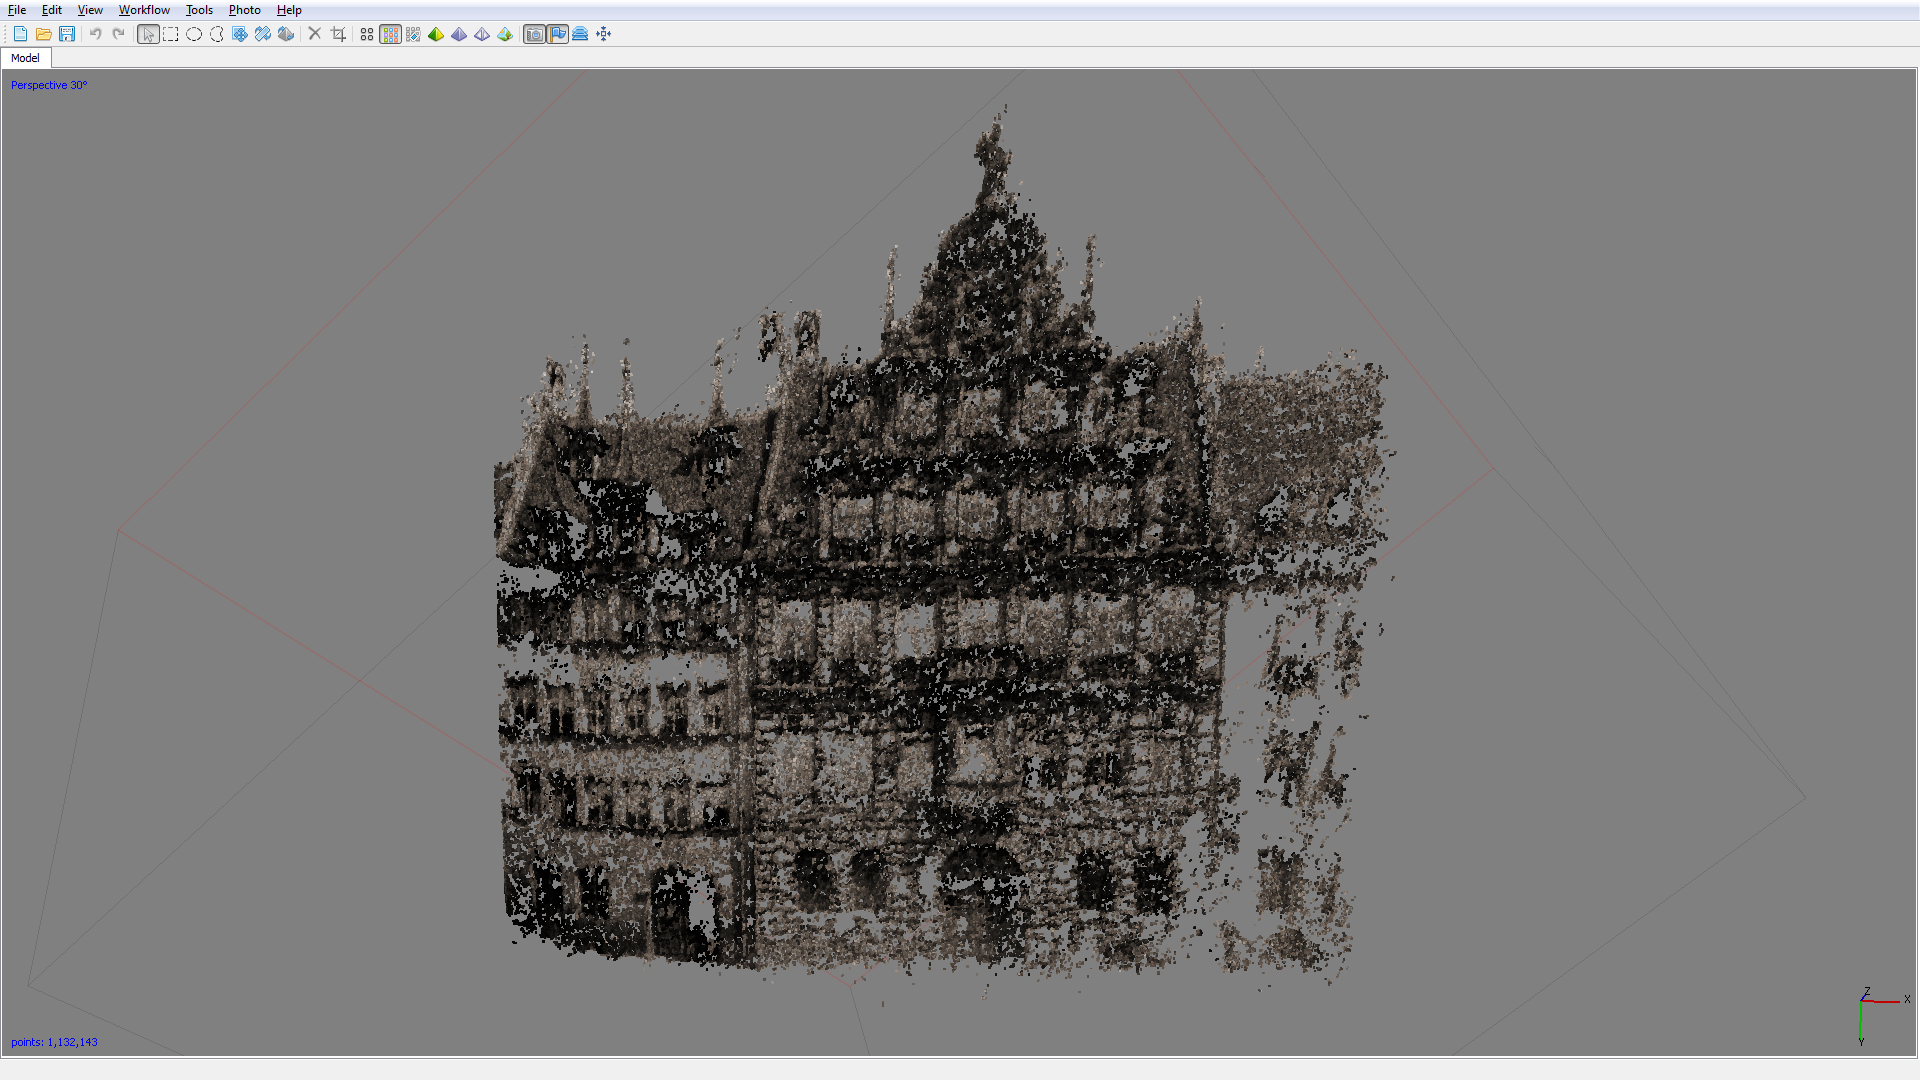
\includegraphics[width=\textwidth]{Production_StereoReconstruction_front.jpg}
		\caption{Historic point cloud front view}
		\label{fig:production_historic_stereo_reconstruction_front}
	\end{subfigure}
	\hfill
	\begin{subfigure}[b]{0.45\textwidth}
		\centering
		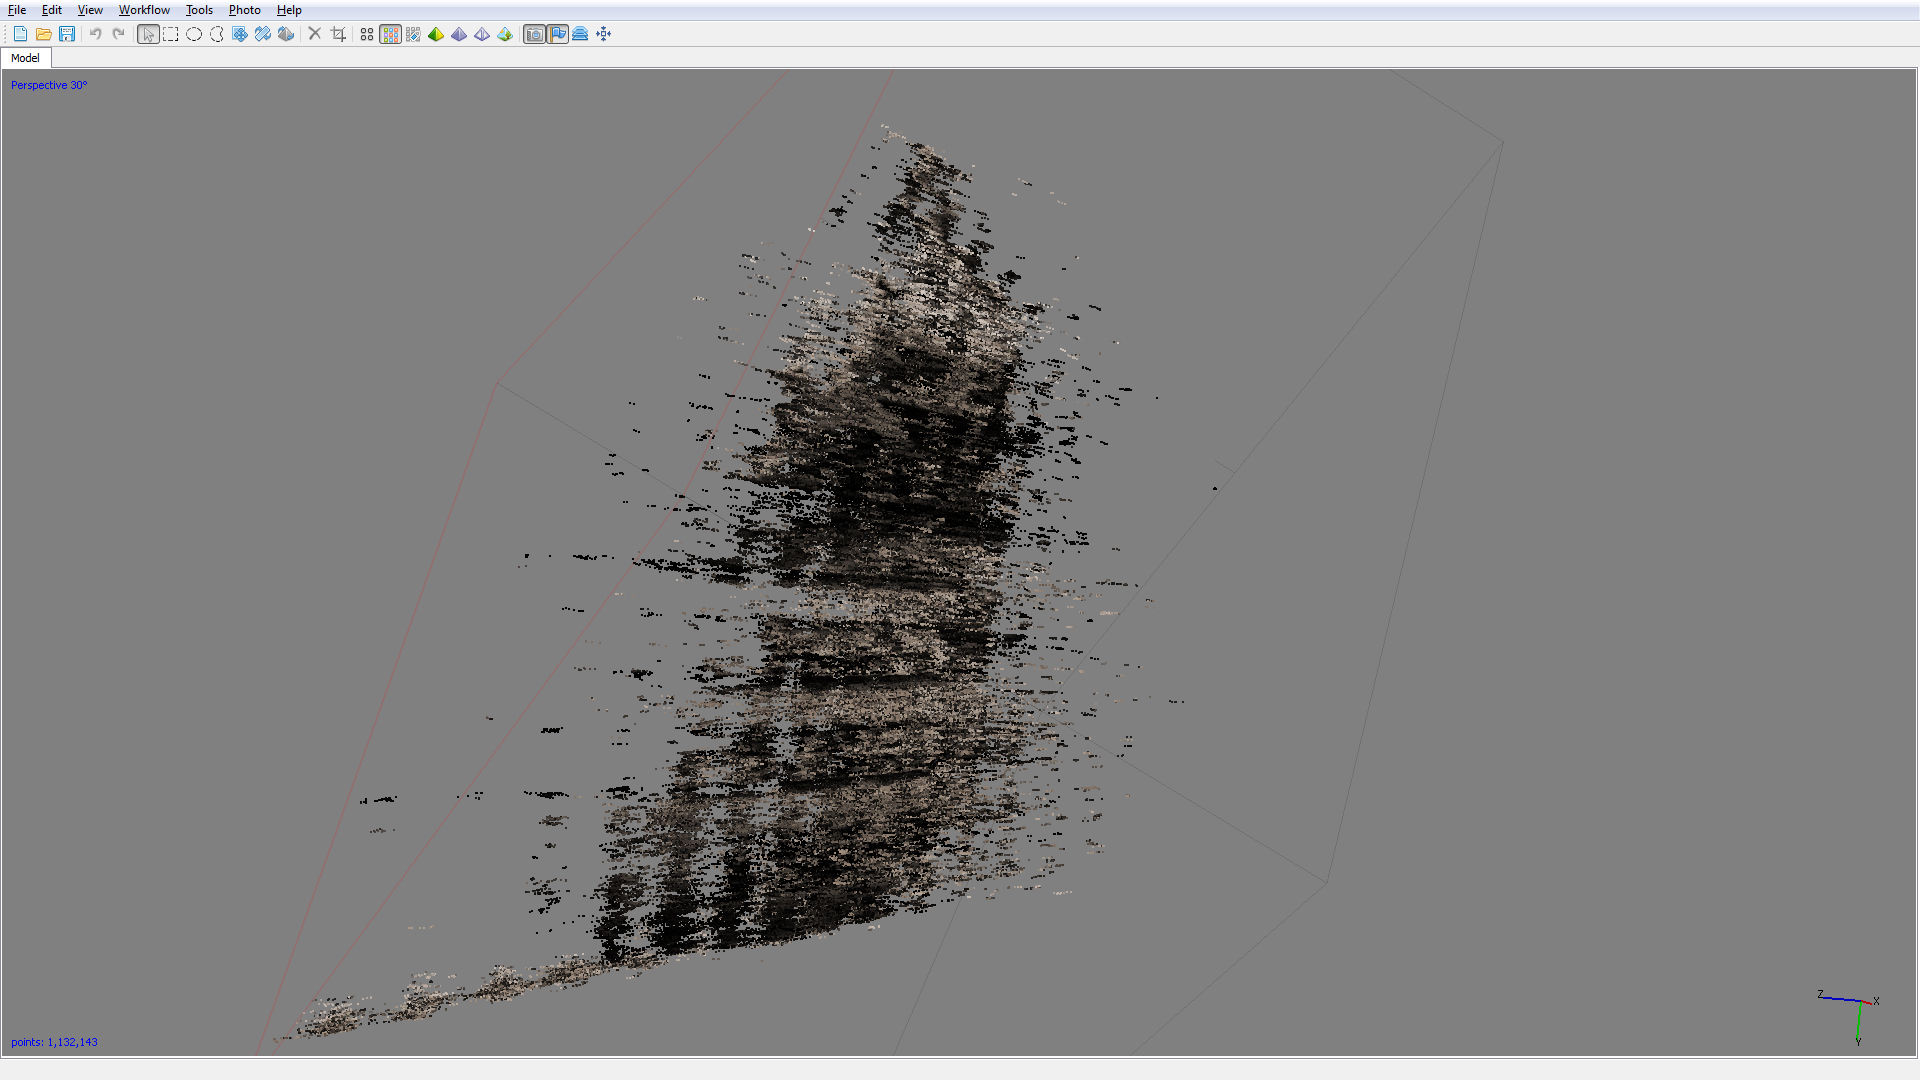
\includegraphics[width=\textwidth]{Production_StereoReconstruction_side.jpg}
		\caption{Historic point cloud right side view}
		\label{fig:production_historic_stereo_reconstruction_side}
	\end{subfigure}
	\caption{Automatic reconstruction results from historic stereo pairs}
	\label{fig:production_historic_stereo_reconstruction}
\end{figure}

The result is quite noisy, but might be suitable for a presentation if viewed carefully with only slight camera movements. However, the results are not satisfying in our view. Hence, they are not suited for the historic 3D reconstruction in this research.

\pagebreak

\section{The finished models}

The manual modeling process took 30 hours and 20 minutes to create the following results:

\begin{figure}[h]
	\centering
	\begin{subfigure}[b]{0.75\textwidth}
		\centering
		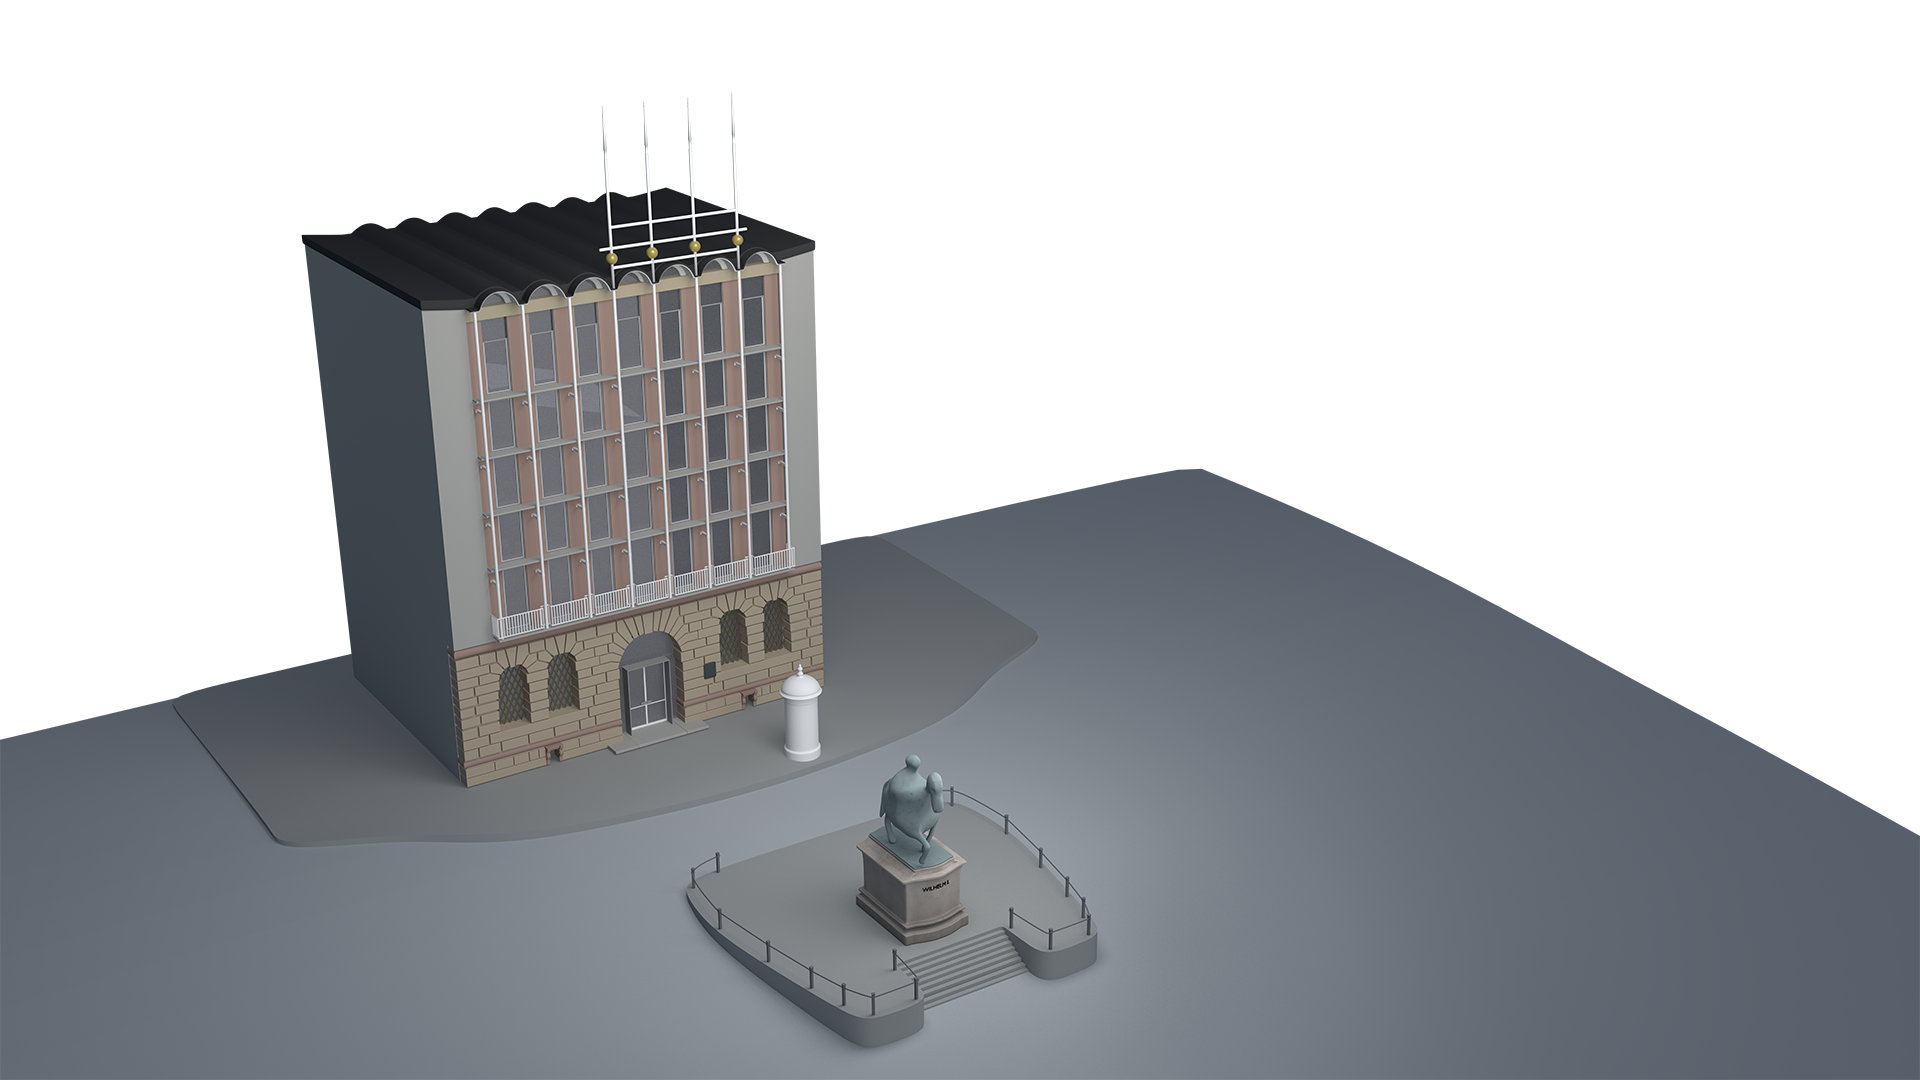
\includegraphics[width=\textwidth]{Pellerhaus_3d_a.png}
		\caption{Modern Pellerhaus}
		\label{fig:pellerhaus_3d_modern}
	\end{subfigure}
	\hfill
	\begin{subfigure}[b]{0.75\textwidth}
		\centering
		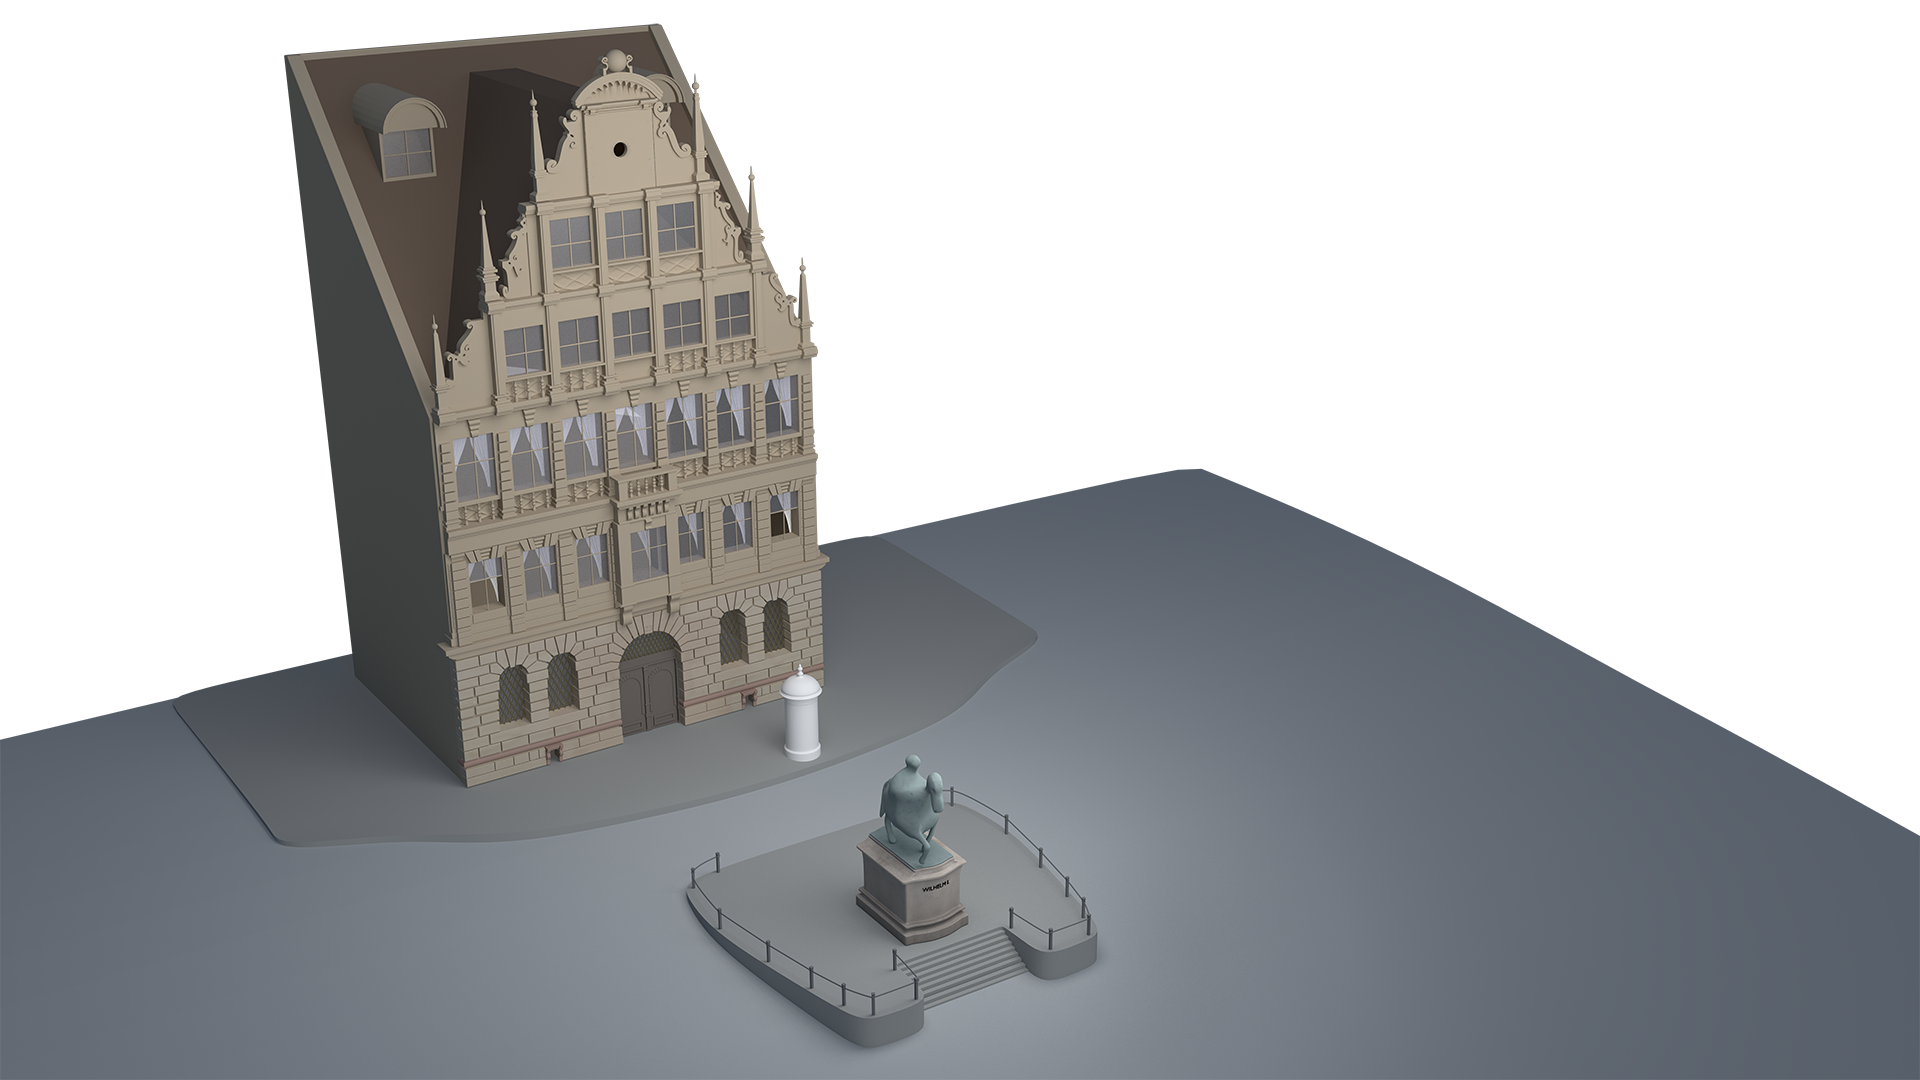
\includegraphics[width=\textwidth]{Pellerhaus_3d_b.png}
		\caption{Historic Pellerhaus}
		\label{fig:pellerhaus_3d_historic}
	\end{subfigure}
	\caption{The finished 3D models of the Pellerhaus}
	\label{fig:pellerhaus_3d_models}
\end{figure}

Rendering took 52 minutes for the modern building model and 54 minutes for the historic model. The render engine Cycles was used at a resolution of 7680 by 4320 pixels and 200 samples.\\

After refining the models, they can be animated to create educational videos about the Pellerhaus history. The historic Pellerhaus can be simulated to fracture and collapse during World War II leaving only debris and major parts of the ground floor. The debris can disappear slowly and the new facade will be created gradually. This may be supported visually by a timeline in the video. Finally, the finished video can be played out in stereoscopic 3D or the models can be 3D printed.\\

Timelapse videos have been created while modeling both buildings and will be published shortly after the research on the project website.
